\section{The models and the optimiser}
\label{sec:models}

\subsection{Classic and prototype neurons}
\label{sec:neurons}

\begin{figure}[t]
\centering
\begin{subfigure}[b]{0.36\textwidth}\centering
\resizebox{\linewidth}{!}{\begin{quantikz}[row sep=0.35cm, column sep=0.45cm]
\lstick{$q_1$ (input)} & \ctrl{2} & \qw & \qw \\
\lstick{$q_2$ (input)} & \qw & \ctrl{1} & \qw \\
\lstick{$q_3$ (neuron)} & \gate{\RX(w_1)} & \gate{\RX(w_2)} & \gate{\RX(b)} \qw
\end{quantikz}}
\caption{Classic neuron (paper, Fig.~1): one controlled rotation per input and a bias
rotation on the neuron's qubit.  The inputs are untouched.}
\end{subfigure}\hfill
\begin{subfigure}[b]{0.6\textwidth}\centering
\resizebox{\linewidth}{!}{\begin{quantikz}[row sep=0.35cm, column sep=0.4cm]
\lstick{$q_1$} & \gate{\RX(\varphi_1)} & \ctrl{2} & \gate{\RX(-\varphi_1)} & \qw & \qw & \qw \\
\lstick{$q_2$} & \qw & \qw & \qw & \gate{\RX(\varphi_2)} & \ctrl{1} & \gate{\RX(-\varphi_2)} \\
\lstick{$q_3$} & \qw & \gate{\RX(\theta)} & \qw & \qw & \gate{\RX(\theta)} & \qw
\end{quantikz}}
\caption{Prototype neuron (paper, Fig.~2): each input is rotated by a learned $\varphi_i$,
controls a rotation by the \emph{same} $\theta$ of the neuron's qubit, and is rotated back.}
\end{subfigure}
\caption{The two neuron types.  A network (paper, Figs.~4, 5, 10, 12) is a layer of
$n_{\mathrm{hid}}$ hidden neurons, each touching all $n_{\mathrm{in}}$ inputs, followed by one
classic output neuron controlled by the hidden qubits.  Our implementation
(\code{ptqnn.circuits.neurons}) builds exactly these gate lists; the un-computation
$\RX(-\varphi_i)$ is what lets several prototype neurons share the same inputs and what lets a
dataset be presented in superposition.}
\label{fig:circuits}
\end{figure}

\Cref{fig:circuits} shows the two neuron types as circuits.  The \emph{classic} neuron is the
quantum perceptron of \cite{snn}: its qubit receives a bias rotation $\RX(b)$ and one controlled
rotation $\CRX(w_i)$ from each input; the inputs are left unchanged.  The \emph{prototype}
neuron rotates input $i$ by $\RX(\varphi_i)$, lets it control a rotation by a shared angle
$\theta$ of the neuron qubit, and rotates it back by $\RX(-\varphi_i)$.  The pair
$(\varphi_1,\dots,\varphi_{n_{\mathrm{in}}})$ is the stored \emph{prototype}: when the input
state is the one that $\RX(-\varphi_i)$ would map to $\ket{1}$ on every qubit, every controlled
rotation fires and the neuron's activation is maximal; when no input matches, none fires and the
activation is zero (\cref{fig:activation}).  A network uses prototype (or, for comparison,
classic) hidden neurons and always a classic output neuron.  Parameter counts: the 11-qubit
bit-count network (5 inputs, 5 hidden) has $5\times(5+1) + (5+1) = 36$ angles; the 7-qubit Flappy
network (2 inputs, 4 hidden) has $4\times 3 + 5 = 17$.

A sanity check that a reader can verify by hand: a single prototype neuron with two inputs,
prototype $(\pi, 0)$ and $\theta = \pi/2$, fed the basis input $(0,1)$, gives $\Pout = 1$; fed
$(1,0)$ it gives $0$; fed $(0,0)$ or $(1,1)$ it gives $\tfrac12$.  \Cref{fig:activation} is this
neuron's activation over all real-valued inputs --- the paper's Fig.~3.  The paper's own surface
bottoms out near $0.2$ rather than $0$, because its parameters (not given) differ from these.

\begin{figure}[t]
\centering
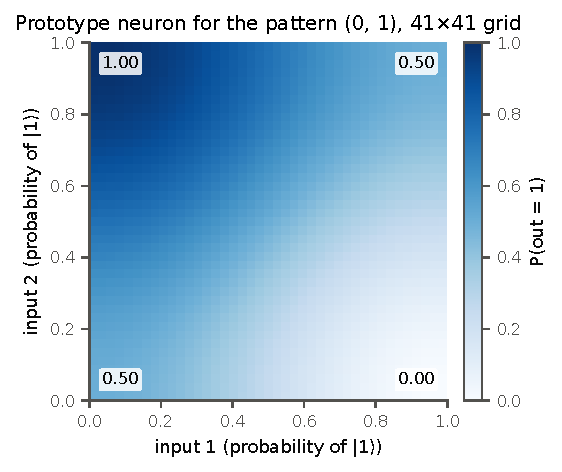
\includegraphics[width=0.46\textwidth]{fig_activation_surface}
\caption{Activation $\Pout$ of one prototype neuron with prototype $(0,1)$ as a function of
the two inputs (each given as the probability that its qubit reads $1$, encoded by
\cref{eq:encoding}).  The corner values are exact.  Run \run{bitcount/20260820T135930Z}.}
\label{fig:activation}
\end{figure}

\subsection{The optimiser: finite differences inside simulated annealing}
\label{sec:kwsa}

The paper trains with no gradient descent.  It estimates the slope of the loss $f$ along one
parameter by the \emph{central difference} $\bigl(f(x+c\,e_i) - f(x-c\,e_i)\bigr)/2c$
(Kiefer--Wolfowitz \cite{kw}), proposes a step against it, and accepts or rejects the proposal by
the \emph{Metropolis rule} of simulated annealing: always accept a decrease of the loss, accept
an increase $\Delta$ with probability $e^{-\Delta/kT}$ at temperature $T$ (paper, Eq.~(3)),
cooling $T$ geometrically.  Neither paper gives the step sizes $a_n$ and $c_n$, the
temperature schedule or what one ``iteration'' is, so the following is our choice (listed in
\cref{app:assumptions}): $a_n = a_0/(n+1)^{0.602}$, $c_n = c_0/(n+1)^{0.101}$ (Spall's standard
exponents \cite{spall}); one \emph{sweep} visits every parameter once in random order, evaluates
the two probes $x\pm c_n e_i$ and the proposed step, and puts the best of the three to the
Metropolis rule.  One sweep therefore costs $3\times(\text{number of parameters})$ circuit
evaluations --- $108$ for the bit-count network.  Whole-vector steps (one gradient estimate of all
parameters, then one step) stalled near $\KL\approx 10^{-2}$ at every setting tried, so the
coordinate sweep is the default; it is what \cref{fig:convergence} shows.  For a rotating
mini-batch of training episodes (Flappy) the incumbent loss is re-evaluated every sweep, because
comparing a candidate scored on one batch against an incumbent scored on another is meaningless
(\cref{sec:flappy}).

\subsection{Simulators}
\label{sec:simulators}

The reference simulator is plain NumPy (state vectors for noiseless runs, density matrices for
noisy ones) and is the oracle for everything else: an independent density-matrix simulator
written blind by a second agent agrees with it to $10^{-12}$ on random circuits; a C density-matrix
library (\code{orkan}), a Monte-Carlo trajectory simulator for circuits too large for density
matrices (Iris at 17 qubits), a GPU density-matrix backend, and one shared batched state-vector
kernel used by all task-specific fast paths are each tested against it on \emph{full output
distributions}, never only on $\Pout$.  The noise model's idle scheduling reproduces Qiskit's
as-soon-as-possible scheduler delay for delay, and its channels agree with Qiskit~Aer's on a
noisy three-qubit circuit to $2\times 10^{-15}$.
